\let\cleardoublepage\clearpage
\part{Экономика, бизнес и услуги}
IRSTI 06.71.57
\hfill {\bfseries \href{https://doi.org/10.58805/kazutb.v.3.24-526}{https://doi.org/10.58805/kazutb.v.3.24-526}}

\sectionwithauthors{B.M. Pazylkhaiyr}{LOCAL COMMUNITIES' PARTICIPATION IN SUSTAINABLE TOURISM
DEVELOPMENT: MANGYSTAU REGION CASE STUDY}

\begin{center}
{\bfseries B.M. Pazylkhaiyr}

Al-Farabi Kazakh National University, Almaty, Kazakhstan
\end{center}

{\bfseries \textsuperscript{🖂}}Correspondent-author: bauyrzhan.pazylkhaiyr@gmail.com

This study examines the vital role of local community involvement in
promoting sustainable tourism development in
Kazakhstan\textquotesingle s Mangystau region. By applying a SWOT
(strengths, weaknesses, opportunities, threats) analysis, the research
evaluates the effects of community participation on tourism efforts,
highlighting both the challenges and potential advantages. The study
concludes that active engagement by local communities enriches the
authenticity of the tourism experience, helps preserve cultural
heritage, and ensures fair economic distribution. However, the region
encounters significant challenges such as inadequate infrastructure,
limited marketing capabilities, and a shortage of tourism-related skills
among residents. The results underscore the importance of strategic
planning, capacity building, and cooperation among government agencies,
local communities, and private entities to advance sustainable tourism
in Mangystau. This strategy is essential for balancing economic growth
with environmental and cultural conservation, ultimately positioning
Mangystau as a prominent destination for sustainable and cultural
tourism in Central Asia.

{\bfseries Key words:} Mangystau, sustainable tourism, local communities,
Kazakhstan, tourism

\sectionheading{ТУРИЗМНІҢ ТҰРАҚТЫ ДАМУЫНА ЖЕРГІЛІКТІ ҚОҒАМДАСТЫҚТАРДЫҢ ҚАТЫСУЫ:
МАҢҒЫСТАУ ОБЛЫСЫНЫҢ МЫСАЛЫНДА}

\begin{center}
{\bfseries Б.М. Пазылхайыр}

Әл-Фараби атындағы Қазақ ұлттық университеті, Алматы, Қазақстан,

e-mail: bauyrzhan.pazylkhaiyr@gmail.com
\end{center}

Бұл зерттеуде Қазақстанның Маңғыстау облысында туризмнің тұрақты дамуына
жәрдемдесуде жергілікті қауымдастықтардың қатысуының маңызды рөлі
қарастырылады. SWOT талдауының көмегімен (күшті және әлсіз жақтары,
мүмкіндіктері мен қауіптері) зерттеу жергілікті қауымдастықтардың
қатысуының туристік қызметке әсерін бағалайды, проблемалар да, ықтимал
артықшылықтар да ерекшеленеді. Мақала жергілікті қауымдастықтардың
белсенді қатысуы туристік тәжірибені байытады, мәдени мұраны сақтауға
көмектеседі және әділ экономикалық бөлуді қамтамасыз етеді деген
қорытындыға келді. Алайда, аймақ инфрақұрылымның жеткіліксіздігі,
маркетингтің шектеулі мүмкіндіктері және жергілікті тұрғындар арасында
туризмге байланысты дағдылардың жетіспеушілігі сияқты маңызды
қиындықтарға тап болады. Нәтижесінде, Маңғыстауда тұрақты туризмді
ілгерілету үшін стратегиялық жоспарлаудың, әлеуетті арттырудың және
мемлекеттік мекемелер, жергілікті қауымдастықтар мен жеке құрылымдар
арасындағы ынтымақтастықтың маңыздылығын көрсетеді. Бұл стратегия
экономикалық өсу мен қоршаған орта мен мәдениетті сақтау арасындағы
тепе-теңдікті қамтамасыз ету үшін қажет, бұл сайып келгенде Маңғыстауды
Орталық Азиядағы тұрақты және мәдени туризмнің көрнекті бағыты ретінде
көрсетеді.

{\bfseries Түйін сөздер:} Маңғыстау, тұрақты туризм, жергілікті
қауымдастықтар, Қазақстан, туризм

\sectionheading{УЧАСТИЕ МЕСТНЫХ СООБЩЕСТВ В УСТОЙЧИВОМ РАЗВИТИИ ТУРИЗМА: НА
ПРИМЕРЕ МАНГИСТАУСКОЙ ОБЛАСТИ}

\begin{center}
{\bfseries Б.М. Пазылхайыр}

Казахский национальный университет им. аль-Фараби, Алматы, Казахстан,

e-mail: bauyrzhan.pazylkhaiyr@gmail.com
\end{center}

В данном исследовании рассматривается важная роль участия местных
сообществ в содействии устойчивому развитию туризма в Мангистауской
области Казахстана. С помощью SWOT-анализа (сильные и слабые стороны,
возможности и угрозы) в исследовании оценивается влияние участия местных
сообществ на туристическую деятельность, выделяются как проблемы, так и
потенциальные преимущества. В исследовании делается вывод о том, что
активное участие местных сообществ обогащает туристический опыт,
помогает сохранить культурное наследие и обеспечивает справедливое
экономическое распределение. Однако регион сталкивается со значительными
проблемами, такими как неразвития инфраструктура, ограниченные
маркетинговые возможности и нехватка навыков, связанных с туризмом,
среди местных жителей. Результаты подчеркивают важность стратегического
планирования, наращивания потенциала и сотрудничества между
государственными учреждениями, местными сообществами и частными
структурами для продвижения устойчивого туризма в Мангистау. Эта
стратегия необходима для обеспечения баланса между экономическим ростом
и сохранением окружающей среды и культуры, что в конечном итоге
позиционирует Мангистау как выдающееся направление устойчивого и
культурного туризма в Центральной Азии.

{\bfseries Ключевые слова:} Мангистау, устойчивый туризм, местные
сообщества, Казахстан, туризм

\begin{multicols}{2}
{\bfseries Introduction.} Sustainable tourism development focuses on
ensuring that tourism\textquotesingle s benefits are fairly distributed
among all stakeholders while minimizing its adverse effects on the
environment, culture, and society. In emerging tourism areas like
Mangystau, Kazakhstan, the active involvement of local communities is
crucial to meet sustainable tourism goals. This article delves into the
role of local communities in the sustainable tourism development of
Mangystau, utilizing a SWOT (Strengths, Weaknesses, Opportunities,
Threats) analysis to thoroughly explore their participation and
potential outcomes {[}1-3{]}.

Situated in southwestern Kazakhstan, the Mangystau region is a place of
striking natural beauty, rich historical significance, and unique
cultural heritage. Renowned for its vast deserts, dramatic landscapes,
and ancient monuments, the region holds significant potential for
tourism development. However, with the growing global emphasis on
environmental sustainability, it is essential that the
region\textquotesingle s tourism growth aligns with sustainable
principles. This article delves into the challenges and opportunities
associated with fostering sustainable tourism in Mangystau {[}4,5{]}.

Achieving sustainable development requires a balanced approach across
economic, environmental, and social dimensions, though different
societies and communities may have varying perspectives on how to
achieve this. The World Tourism Organization, for instance, has set
guidelines that aim to balance the needs of the tourism sector with
environmental protection and cultural heritage preservation. These
guidelines promote sustainability principles, such as making tourist
attractions accessible to all and assigning responsibility for their
upkeep to local governments and communities. Additionally, a portion of
tourism revenue should be reinvested in maintaining and improving these
sites. Tourism strategies should also focus not only on immediate
financial returns but also on long-term plans for protecting cultural
heritage {[}6,7{]}.

However, achieving this balance in practice is often difficult. Many
small businesses in the tourism industry focus on short-term profits at
the expense of environmental and cultural preservation. At the same
time, politicians may implement environmental regulations to maintain
their political standing, yet still permit tourism developments that
damage the environment and local culture. Therefore, it is crucial for
stakeholders in the tourism sector---such as businesses, agencies, NGOs,
and local communities---to participate in the development process. While
this collaboration is challenging, if these groups can agree on a common
vision, they can move toward sustainable tourism that maintains balance
across all elements. Nonetheless, involving local communities in the
long-term planning of tourism is difficult, as they often face negative
impacts from business activities. Reaching a consensus that ensures
fairness across all aspects of sustainable tourism remains a significant
challenge {[}6,8{]}.

Sustainable tourism is often viewed as a more considerate approach to
tourism, characterized by small-scale operations that are sensitive to
the natural environment. This concept emphasizes the importance of
minimizing tourism\textquotesingle s impact on both culture and the
environment, while also ensuring that the local community is actively
involved, particularly in decision-making processes. As the strategies
for park protection have evolved, it has become increasingly important
to address sustainable tourism development. In many academic
discussions, sustainable development models frequently highlight the
need for stakeholder collaboration, with a particular focus on involving
local communities from the early development stages {[}9, 10{]}.

Kazakhstan is actively pursuing sustainable development across three
main areas: social, economic, environmental. The country has outlined
specific actions for these initiatives to the international community
and played a significant role in the United Nations summit in 2015.
Kazakhstan has established a comprehensive legal framework for
environmental protection, which includes over 200 additional regulatory
documents and around ten laws. The introduction of the Ecological Code
in 2007 led to the repeal of several earlier laws, such as "On
Environmental Protection," "On Atmospheric Air Protection," and "On
Ecological Expertise." Nevertheless, current executive activities still
rely on previously established bylaws. Additionally, there is a notable
lack of legislation requiring environmental audits, waste management for
production and consumption, or mandatory environmental insurance
{[}11-12{]}.

{\bfseries Materials and methods.} This research examines the role of
active community involvement in the sustainable tourism development of
the Mangystau region, with a focus on the key factors that either
facilitate or obstruct this process. The hypothesis posits that local
community participation is essential for achieving sustainable tourism,
as it enhances the authenticity of the tourism experience, preserves
cultural heritage, and ensures fair distribution of economic benefits.
However, the process is hindered by challenges such as inadequate
infrastructure, limited marketing resources, and a lack of
tourism-related skills among community members.

To tackle these challenges, the research will follow a multi-stage
approach, starting with an in-depth literature review on sustainable
tourism, community participation, and the specific conditions in the
Mangystau region to identify relevant theories and frameworks. This will
be followed by a SWOT analysis to assess the internal strengths and
weaknesses, along with the external opportunities and threats related to
local community participation in tourism development. The final stage
will synthesize the findings to draw conclusions on the role of local
communities in sustainable tourism, resulting in a comprehensive report
that includes the SWOT analysis, key insights, and strategic
recommendations. Several authors, as Huang and Wei (2024) Cankül et al.
(2024) Uchiyama and Kohsaka (2021) have used SWOT analysis method in
their work {[}1-3{]}.

The study is expected to demonstrate that local community participation
is a critical component of sustainable tourism in the Mangystau region.
Anticipated findings include identifying strengths, such as the region's
rich cultural heritage and community knowledge that contribute to
authentic and sustainable tourism experiences; recognizing weaknesses,
like insufficient infrastructure and limited marketing capabilities,
that hinder tourism growth; identifying significant opportunities in
niche tourism markets like eco-tourism and cultural tourism that align
with global trends and benefit the community; and understanding
potential threats, such as environmental degradation and cultural
erosion, which could jeopardize the sustainability of tourism in the
region. These insights will help develop strategic recommendations to
enhance local community participation, address current challenges, and
ensure sustainable tourism development in the Mangystau region. The
author developed a conceptual framework for the research to achieve the
study\textquotesingle s outcome (Fig.1).
\end{multicols}

\begin{figure}[H]
	\centering
	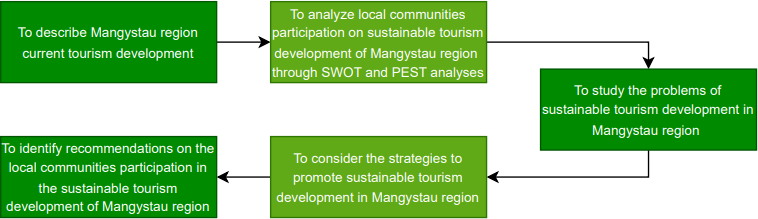
\includegraphics[width=0.8\textwidth]{assets/337}
	\caption*{Fig. 1 - Research conceptual framework}
\end{figure}

\begin{multicols}{2}
\emph{Study field.} Mangystau is located in the southwestern part of
Kazakhstan (Fig. 2), and a region renowned for its rich history,
cultural significance, and natural beauty. The landscape is marked by
vast deserts, unique rock formations, underground mosques, and the
Caspian Sea coastline. Historically, Mangystau served as a critical
crossroads for traders and travelers, leaving behind a rich array of
cultural and archaeological treasures. Despite these natural and
cultural assets, Mangystau remains relatively unknown as a tourist
destination in Kazakhstan, presenting both challenges and opportunities
for sustainable tourism development {[}4,5,13{]}.
\end{multicols}

\begin{figure}[H]
	\centering
	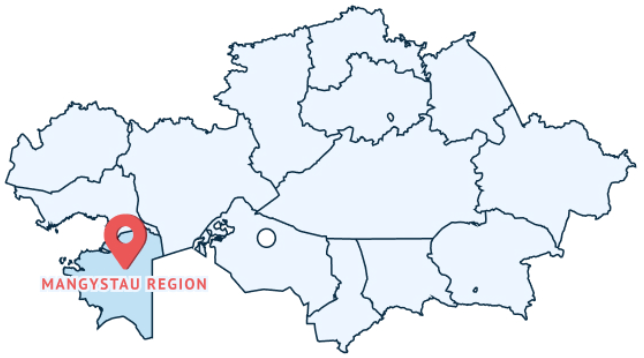
\includegraphics[width=0.5\textwidth]{assets/338}
	\caption*{Fig. 2 -- The location of Mangystau region {[}13{]}}
\end{figure}

\begin{multicols}{2}
The region is home to a diverse population with communities that have
maintained their traditions, languages, and customs for generations.
These communities play a pivotal role in Mangystau's sustainable tourism
strategy, as their participation can significantly enhance the
authenticity and sustainability of tourism initiatives. To maximize this
potential, it is essential to assess the strengths, weaknesses,
opportunities, and threats associated with local community involvement
in tourism.

Table 1 outlines the protected natural areas in the Mangystau region,
highlighting their size, location, and the government bodies responsible
for their management.
\end{multicols}

\begin{table}[H]
\caption*{Table 1 - Mangystau region's specially protected natural areas {[}14{]}}
\centering
\begin{tabular}{|l|p{0.2\textwidth}|p{0.07\textwidth}|p{0.13\textwidth}|p{0.4\textwidth}|}
\hline
№ & The name of specially protected natural areas & Area, hectare & Location & Authority \\ \hline
1 &
  Ustyurt State Nature Reserve &
  223342 &
  Karakiyansky district &
  Forestry and Wildlife Committee Ministry of Ecology, Geology and Natural Resources of the Republic of Kazakhstan \\ \hline
2 &
  Aktau-Buzachinsky State Nature Reserve (zoological) &
  170000 &
  Tupkaragan district &
  Forestry and Wildlife Committee Ministry of Ecology, Geology and Natural Resources of the Republic of Kazakhstan \\ \hline
3 &
  Karakiya-Karakol State Nature Reserve (zoological) &
  137500 &
  Karakiyansky district &
  Forestry and Wildlife Committee Ministry of Ecology, Geology and Natural Resources of the Republic of Kazakhstan \\ \hline
4 &
  Kenderli-Kayasan State Protected Area &
  1230290 &
  Karakiyansky district &
  Forestry and Wildlife Committee Ministry of Ecology, Geology and Natural Resources of the Republic of Kazakhstan \\ \hline
5 &
  Mangyshlak Experimental Botanical Garden &
  39 &
  Aktau city &
  Science Committee of the Ministry of Science and Higher Education of the Republic of Kazakhstan \\ \hline
\end{tabular}
\end{table}

\begin{figure}[H]
	\centering
	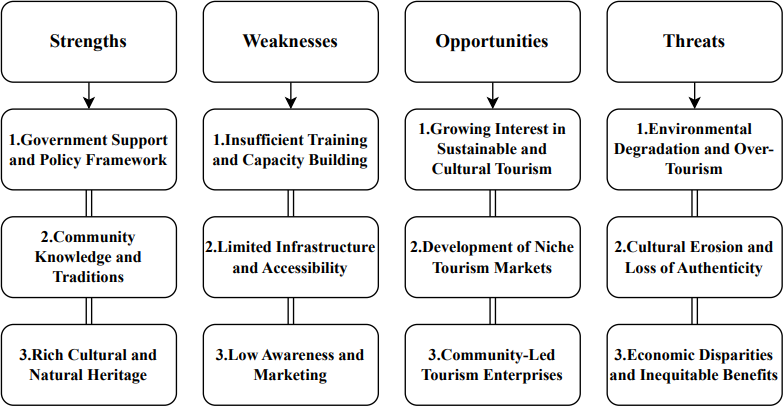
\includegraphics[width=0.9\textwidth]{assets/339}
	\caption*{Fig. 3 -- SWOT analysis result {[}2{]}}
\end{figure}

\begin{multicols}{2}
{\bfseries Results and discussion.} By utilizing the SWOT framework, the
research will systematically evaluate the internal and external factors
affecting sustainable tourism in the Mangystau region. Additionally,
existing data from government reports, academic journals, and industry
publications will be analyzed to support the primary data findings.

Fig. 3 offers a SWOT analysis of tourism development, emphasizing
strengths such as government backing and cultural richness, while also
noting weaknesses like limited training and infrastructure. It outlines
opportunities in sustainable tourism and community-driven initiatives,
and recognizes threats including environmental damage and cultural loss.
This analysis provides a strategic perspective on factors affecting
tourism development {[}15{]}.

\emph{Strengths.} The Kazakh government prioritizes tourism for economic
diversification and has implemented policies to promote sustainable
tourism, including investments in infrastructure and eco-friendly
practices. Mangystau is rich in cultural landmarks, including the
Beket-Ata Underground Mosque, Shakpak-Ata Necropolis, and ancient
petroglyphs. These sites provide a deep insight into the
region\textquotesingle s history and identity, forming a strong
foundation for cultural tourism. The region\textquotesingle s natural
landscapes, such as deserts, cliffs, and the Caspian Sea coastline, are
home to rare species, making it an ideal spot for eco-tourism. Landmarks
like the Karagiye Depression and Ustyurt Plateau attract adventure
tourists and nature enthusiasts. Local communities maintain a rich
cultural heritage through traditional crafts, music, dance, and oral
histories, which can be integrated into tourism to offer visitors an
authentic experience and support local economies. Indigenous knowledge
of the region's natural and cultural resources is crucial for
sustainable tourism. Local guides can share insights into historical
sites, traditional uses of plants, and the spiritual significance of
natural landmarks. Mangystau region has specially protected natural
areas (Table 2), which can be popular places for the tourists.

\emph{Weaknesses.} The region\textquotesingle s vast distances between
attractions, underdeveloped road networks, and lack of public
transportation make it challenging for tourists to explore. The scarcity
of diverse accommodations and essential services like restaurants and
visitor centers further limits tourism growth. Mangystau is not widely
recognized as a tourist destination, and local communities often lack
the resources and expertise for effective marketing. This hinders the
region's ability to attract tourists and generate revenue. Many locals
have limited experience in tourism, particularly in hospitality and
foreign languages. Although some training programs exist, ongoing
education is needed to meet industry standards and support sustainable
tourism development.

\emph{Opportunities.} With increasing global interest in sustainable and
cultural tourism, Mangystau's rich heritage and diverse ecosystems
position it well to attract tourists seeking authentic and eco-friendly
experiences. The region\textquotesingle s rugged landscapes are ideal
for adventure tourism, while its religious sites can draw pilgrims.
There is also potential for health and wellness tourism, leveraging
natural hot springs and tranquil environments. Empowering local
communities through tourism enterprises ensures that the economic
benefits are shared equitably. Social enterprises and cooperatives can
create jobs for marginalized groups and reinvest profits into community
development.

\emph{Threats.} Without careful management, tourism growth could lead to
environmental degradation, over-tourism, and strain on infrastructure.
Waste and pollution are particular concerns, especially in remote areas
with limited infrastructure. The commercialization of cultural practices
for tourism can lead to a loss of authenticity and cultural erosion. It
is essential to preserve the region's cultural identity while promoting
tourism. Over-reliance on tourism as a primary economic driver can make
local communities vulnerable to external shocks, such as economic
downturns or natural disasters. Diversifying the economy and developing
resilience strategies are necessary for long-term stability.

\emph{Problems in Developing Sustainable Tourism.} The environment of
Mangystau is defined by fragile desert ecosystems that are highly
vulnerable to damage. The region\textquotesingle s arid climate and
limited water resources make it especially susceptible to the impacts of
tourism. Unregulated tourism activities can result in pollution, habitat
destruction, and the depletion of these scarce natural resources.
Achieving a balance between tourism development and the preservation of
these sensitive ecosystems is a major challenge {[}16{]}.

Mangystau currently lacks the infrastructure needed to support a
significant increase in tourist numbers. The region\textquotesingle s
roads, public transportation, accommodations, and waste management
systems are underdeveloped, making it challenging to meet the needs of
both tourists and local residents. Developing this infrastructure in a
sustainable way requires substantial investment and careful planning to
ensure it meets regional needs without exacerbating environmental issues
{[}17-18{]}.

Developing sustainable tourism requires a solid understanding of
environmental conservation and community involvement. In Mangystau,
there is a lack of local expertise in sustainable tourism practices,
which can hinder the effective implementation of such initiatives.
Additionally, without proper education and training, local communities
may not fully benefit from tourism or might unintentionally contribute
to environmental degradation.
\end{multicols}

\begin{table}[H]
\caption*{Table 2 -- Strategic Framework for Sustainable Tourism Development in Mangystau}
\centering
\begin{tabular}{|p{0.2\textwidth}|p{0.25\textwidth}|p{0.25\textwidth}|p{0.2\textwidth}|}
\hline
Strategic Objective &
  Action Steps &
  Expected Outcome &
  Key Stakeholders \\ \hline
Enhance Infrastructure &
  Upgrade roads, develop eco-lodges, improve public transportation &
  Increased accessibility and comfort for tourists &
  Government, private sector, local communities \\ \hline
Promote Cultural Heritage &
  Create and promote cultural festivals, invest in preserving historic sites &
  Increased tourist interest in cultural sites, preservation of traditions &
  Government, local communities, NGOs \\ \hline
Develop Niche Markets &
  Identify and promote adventure tourism, health and wellness tourism, and religious tourism &
  Diversification of tourism offerings, attraction of niche markets &
  Tourism operators, local entrepreneurs, international marketing partners \\ \hline
Foster Community-Led Enterprises &
  Provide training and financial support for community-run guesthouses, craft cooperatives, and guided tours &
  Increased community empowerment, equitable distribution of tourism benefits &
  {\ul Local communities, NGOs, microfinance institutions} \\ \hline
Ensure Environmental Sustainability &
  Implement strict waste management protocols, limit visitor numbers in sensitive areas, promote eco-friendly tourism activities &
  Preservation of natural resources, reduction of tourism-related degradation &
  Environmental agencies, local communities, eco-tourism organizations \\ \hline
Marketing and Global Awareness &
  Develop a comprehensive digital marketing strategy, engage with international travel bloggers, and partner with global eco-tourism organizations &
  Improved global and domestic recognition of Mangystau as a tourist destination &
  Government, digital marketing firms, international tourism bodies \\ \hline
\end{tabular}
\end{table}

\begin{multicols}{2}
While sustainable tourism seeks to balance economic development with
environmental and cultural preservation, this balance can be difficult
to achieve. The initial costs of creating sustainable infrastructure and
training programs can be high and the financial returns may not be
immediate. Moreover, ensuring that tourism generates sufficient income
to support local communities without overexploiting resources requires
careful management.

Mangystau is home to a rich cultural heritage with deep-rooted
traditions and customs. If not managed carefully, the influx of tourists
can lead to the erosion of these cultural values and practices. There is
a risk that tourism could commercialize or exploit cultural elements,
resulting in a loss of authenticity. It is crucial to ensure that
tourism development respects and preserves local culture for sustainable
growth {[}16,18{]}.

\emph{Strategic Framework for Sustainable Tourism Development.}
Sustainable tourism in Mangystau is a powerful tool for environmental
protection, economic development, and cultural preservation, with local
communities playing a central and indispensable role in its success. The
enhancement of infrastructure, such as roads and eco-lodges, not only
makes the region more accessible and comfortable for tourists but
directly benefits local communities, who are crucial to the development
process. By actively participating in promoting cultural heritage
through festivals and the preservation of historic sites, local
residents are empowered to take pride in their traditions, sharing them
with visitors while safeguarding these cultural elements from
disappearing (Table 2).

The development of niche markets, including adventure, wellness, and
religious tourism, provides local entrepreneurs with unique
opportunities to create and offer experiences that are deeply rooted in
the region\textquotesingle s distinct characteristics. Community-led
enterprises, such as guesthouses, craft cooperatives, and guided tours,
ensure that the economic benefits of tourism are distributed equitably
among residents, enhancing community empowerment and fostering a strong
sense of ownership over Mangystau's natural and cultural resources.

Environmental sustainability is another critical pillar, with local
communities playing a vital role in implementing eco-friendly practices
like strict waste management and controlling visitor numbers in
sensitive areas. This collaboration helps preserve
Mangystau\textquotesingle s unique landscapes and biodiversity,
attracting environmentally conscious tourists and contributing to
long-term economic stability that benefits the community.

A comprehensive digital marketing strategy, involving local communities
and connecting with international travel bloggers and global eco-tourism
organizations, can significantly boost Mangystau's recognition as a
premier tourist destination. This not only stimulates the local economy
but also ensures that tourism development aligns with the values and
needs of the residents. By involving local communities in every aspect
of tourism planning and development, sustainable tourism in Mangystau
guarantees that economic growth, cultural preservation, and
environmental protection are achieved in a way that prioritizes the
well-being of current residents and secures a thriving future for
generations to come. This community-centered approach helps prevent the
adverse effects of over-tourism, such as environmental degradation and
cultural erosion, and supports the creation of a resilient tourism
industry that meets the long-term needs of the region and its people.

{\bfseries Conclusion.} The Mangystau region of Kazakhstan offers a unique
opportunity for sustainable tourism development, where the active
participation of local communities is both vital and necessary. The SWOT
analysis reveals that while the region has considerable strengths in its
cultural and natural heritage, it also faces significant challenges
related to infrastructure, marketing, and capacity building.

Sustainable tourism involves the planning and management of tourism
activities in a way that ensures the long-term preservation of the
environment, promotes social equity, and supports economic
sustainability. It focuses on reducing negative impacts on the
environment and local communities while maximizing benefits for all
involved. In Mangystau, sustainable tourism would mean protecting the
region\textquotesingle s natural and cultural assets while promoting
economic development and enhancing the well-being of local residents.

The tourism industry in Mangystau is still in its early stages. The
region is home to attractions like the Ustyurt Plateau, the coastline of
the Caspian Sea, the Karagiye Depression, and various historical sites
such as the underground mosques of Beket-Ata and Shakpak-Ata. Despite
these attractions, the region has yet to emerge as a prominent tourist
destination, primarily due to inadequate infrastructure, accessibility
challenges, and limited promotional efforts.

The sustainable development of tourism in Mangystau hinges on active
local participation, as the region faces numerous environmental,
cultural, and economic challenges. The delicate desert ecosystems are
particularly vulnerable to the adverse effects of uncontrolled tourism,
which can lead to pollution, habitat destruction, and resource
depletion. Addressing these issues requires thoughtful investment in
sustainable infrastructure, such as eco-friendly accommodations and
efficient waste management systems.

\begin{itemize}
\item
  Cultural preservation is also paramount, given
  Mangystau\textquotesingle s rich heritage. By involving local
  communities in tourism planning, the region can ensure that
  development respects and promotes its cultural traditions.
  Community-based tourism can empower residents by providing alternative
  sources of income and fostering cultural exchange.
\item
  Eco-tourism and cultural tourism present significant opportunities for
  Mangystau, attracting visitors who value environmental conservation
  and cultural appreciation. The Kazakhstan government, in collaboration
  with the private sector, can support these initiatives by enacting
  policies that promote sustainability and by providing incentives for
  eco-friendly businesses.
\item
  Public-private cooperation is crucial for financing infrastructure
  projects and ensuring equitable distribution of tourism benefits.
  Additionally, raising awareness about sustainable tourism practices
  among tourists, local communities, and businesses is essential for
  fostering a culture of sustainability.
\item
  Finally, ongoing research and monitoring are necessary to track the
  impact of tourism on the environment and local communities, enabling
  data-driven decision-making to address emerging challenges.
\end{itemize}

Local participation is key to ensuring that tourism development in
Mangystau is not only economically beneficial but also environmentally
and culturally sustainable.

To achieve sustainable tourism development, it is crucial to address
these weaknesses and threats through strategic planning, capacity
building, and active community involvement. Empowering local communities
to take ownership of tourism initiatives, providing them with the
necessary skills and resources, and ensuring that tourism development
aligns with their cultural values and environmental concerns are vital
steps toward a sustainable and inclusive tourism future for Mangystau.

By leveraging the region's strengths and capitalizing on new
opportunities, Mangystau can establish itself as a leading destination
for sustainable and cultural tourism in Central Asia. However, this will
require a collaborative effort between local communities, government
agencies, and international partners to create a tourism model that not
only attracts visitors but also preserves the region's cultural and
natural heritage for future generations. The success of sustainable
tourism in Mangystau ultimately hinges on the ability of all
stakeholders to work together toward shared goals, ensuring that tourism
benefits are equitably distributed and that the region\textquotesingle s
unique cultural and environmental assets are protected and celebrated.

The development of sustainable tourism in the Mangystau region presents
significant challenges as well as promising opportunities. Although the
region faces environmental, infrastructural, and cultural obstacles, the
potential benefits of sustainable tourism---including environmental
protection, economic growth, cultural preservation, community
empowerment, and long-term sustainability---are substantial. By
addressing these challenges and leveraging the advantages, Mangystau can
create a tourism industry that not only attracts visitors but also
preserves the region\textquotesingle s heritage.

Developing sustainable tourism in the Mangystau region presents a
promising opportunity for economic growth, environmental protection, and
cultural preservation. By adopting a comprehensive approach, that
balances the needs of tourists, local communities, and the environment,
Mangystau has the potential to become a leading example of sustainable
tourism in Kazakhstan and beyond. With the right strategies and
investments, the region can attract international visitors while
safeguarding its unique heritage for future generations.

\emph{{\bfseries Financing.} This research was funded by the Science
Committee of the Ministry of Science and Higher Education of the
Republic of Kazakhstan (Grant No. BR21882122 ``Sustainable Development
of Natural-Industrial and Socio-Economic Systems of the West Kazakhstan
Region in the Context of Green Growth: A Comprehensive Analysis,
Concept, Forecast Estimates and Scenarios'').}
\end{multicols}

\begin{center}
{\bfseries References}
\end{center}

\begin{noparindent}
1.
  Huang T., Wei J. Management strategies for museum night opening in
  China: a SWOT-TOWS analysis of Shanghai museums // Cogent Social
  Sciences. -2024. -Vol. 10(1). DOI:10.1080/23311886.2024.2327857

2.
  Cankül D., Cankül I., Aktepe B. Meal sharing economy: evaluation with
  SWOT analysis from host and local food tourists perspectives //
  Journal of Foodservice Business Research. -2024. -P. 1--22. DOI:
  10.1080/15378020.2024.2387388

3.
  Uchiyama Y., Kohsaka R. Strategies of Destination Management
  Organizations in Urban and Rural Areas: Using Text Analysis Method for
  SWOT Descriptions at Meta-level // International Journal of
  Hospitality \& Tourism Administration. -2021. -Vol. 24(1). -P.
  123-141. DOI:

10.1080/15256480.2021.1953422

4.
  Ämırbaeva A.A., Ryskulov S.K., Ahmetova K.A. Qazaqstannyñ Mañğystau
  oblysynyñ auyldyq turizmınıñ äleuettı resurstary.~Agrarlyq naryq
  problemalary. -2023. --Vol. 2.
  -P.71-80.~https://doi.org/10.46666/2023-2.2708-9991.07 {[}in Kazakh{]}

5.
  Sabirova R.K., Andabaeva G.K., Mahanova A.N. Mañğystau öñirinde turizm
  türlerin damytu jäne onyñ auyldyq aumaqtardy damytuğa äseri.~Central
  Asian Economic Review. -2022(5), -P.142-154.
  
  https://doi.org/10.52821/2789-4401-2022-5-142-154 {[}in Kazakh{]}

6.
  Morea, J. P. Environmental justice, well-being and sustainable tourism
  in protected area management. Journal of Ecotourism. -2021. -Vol.
  20(3). -P. 250-269. DOI:10.1080/14724049.2021.1876072

7.
  Prayitno G. et al. Social capital for sustainable tourism development
  in Indonesia // Cogent Social Sciences. -2023. -Vol. 10(1).
  DOI:10.1080/23311886.2023.2293310

8.
  Nyiwul L. et al. Adoption of tools for sustainable tourism
  development: role of environmental vulnerability // Journal of Policy
  Research in Tourism Leisure and Events. -2024. -P. 1--23.
  
  https://doi.org/10.1080/19407963.2024.2317908

9.
  Hossain M.I., Kumar J., Islam Md.T. Antecedents of Sustainable Tourism
  Development in Sundarbans, Bangladesh with the Moderation of Political
  Instability and Mediation of Destination Resilience // Tourism
  Planning \& Development. -2024. -P. 1--29.
  DOI:10.1080/21568316.2024.2347222

10.
  Gani, A., Khairil, A., Mohamad, A., Samdin, Z. Attributes of
  successful public participation in planning for sustainable tourism in
  protected areas: A modified delphi study. -2015. --Vol. 23. --P.
  49-64.

11.
  Altaibayeva, Z., Pfeifer N., Shelomentseva V. \& Khamzina Sh.
  Assessment of the attractiveness and problems of the Territorial
  Natural Recreational Systems of North-East Kazakhstan by the
  population // Bulletin of the Karaganda University. Economy series.
  -2021. -Vol. 4(104), -P. 4-12. DOI:
  
  https://doi.org/10.31489/2021ec4/4-12

12.
  Pazylkhaiyr B., Assipova Zh.M., Bertocchi D. Development of tourism
  environmental management in Kazakhstan based on successful
  international experience // Bulletin of the Karaganda university
  economy series. -2023. -Vol. -110(2). -P. 79--89. DOI
  10.31489/2023Ec2/79-89

13.
  Welcome.kz. Unknown Mangystau Off-Road Tour -2024. {[}Online{]}.
  Available:
  
  https://welcome.kz/en/adventure/off-road-tours/unknown-mangystau-off-road
  {[}Accessed: Aug. 24, 2024{]}.

14.
  Adilet. Ob utverjdenii perechnya osobo ohranyaemih prirodnih
  territorii respublikanskogo znacheniya. -2017. {[}Online{]}.
  Available: https://adilet.zan.kz/rus/docs/P1700000593 {[}Accessed:
  Aug. 24, 2024{]}.

15.
  Font-Barnet A., Andreu M.N.-L. Research on tourism, well-being, and
  nature: a bibliometric analysis // Anatolia an International Journal
  of Tourism and Hospitality/Anatolia an International Journal of
  Tourism and Hospitality Research. -2021. -Vol. 34, -№ 2. -P. 163--175.
  DOI:10.1080/13032917.2021.2002699

16.
  Harish P., Rao Y.V. Research on sustainable tourism and biodiversity:
  a bibliometric analysis // Anatolia. -2024. -P. 1--21.

17.
  Kusumawardhani Y. et al. Smart tourism practice in the scope of
  sustainable tourism in emerging markets: a systematic literature
  review // Cogent Social Sciences. -2024. -Vol. 10(1).

  DOI:10.1080/23311886.2024.2384193

18.
  Niewiadomski P., Mellon V. Transitioning towards sustainable tourism
  in the Outer Hebrides: an evolutionary investigation // Tourism
  Geographies. -2023. -Vol. 26(2). -P. 214--236. DOI

  10.1080/14616688.2023.2283730
\end{noparindent}

\emph{{\bfseries Information about the author}}

\begin{noparindent}
Pazylkhaiyr B.M. -- Senior teacher of Department of Recreation geography
and tourism, Research Fellow, Al-Farabi Kazakh National University,
Almaty, Kazakhstan, e-mail: bauyrzhan.pazylkhaiyr@gmail.com.
\end{noparindent}

\emph{{\bfseries Сведения об авторах}}

\begin{noparindent}
Пазылхайыр Б.М. -- старший преподаватель кафедры рекреационной географии
и туризма, научный сотрудник, Казахский национальный университет им.
аль-Фараби, Алматы, Казахстан, e-mail: bauyrzhan.pazylkhaiyr@gmail.com.
\end{noparindent}

